\section{生理学基础与信号特征}
\label{sec:physio}

\subsection{PPG原理与测量条件}
\label{sec:ppg_principle}

PPG 信号是由发光二极管照射皮肤，再由传感器接收透射或反射光强得到的信号。心脏射血期动脉血容量增加，血红蛋白对光的吸收增强，接收光强随之下降，形成上升支；舒张期血液回流、血容量减少，光强回升，形成下降支\cite{allen2007photoplethysmography}。采集到的信号可分解为随心跳搏动的交流（AC）分量与缓慢漂移的直流（DC）分量：前者反映搏动性灌注，后者由皮肤、静脉血与佩戴压力共同决定。PPG本质上是血容量脉搏的光学观测，而非动脉压力波形本身\cite{reisner2008utility}。

另外，测量条件会系统性地影响波形。波长决定探测深度，绿光主要反映浅层毛细血管的容积变化，近红外光可穿至更深的皮下小动脉；测量部位决定光路形式，指端多为透射式，腕部与耳部则为反射式；接触压力过大将压迫血管、过小则光耦合不足，两者都会压低 AC 幅度并使形态失真\cite{allen2007photoplethysmography}。这些差异意味着不同设备、不同佩戴位置采集的波形并非同一分布，是\cref{sec:challenges}中跨设备泛化问题的来源之一。

\subsection{波形形态与特征点}
\label{sec:ppg_morphology}

如\cref{fig:ppg_wave}所示，一个心动周期的波形通常呈双峰形态：主峰之后，来自外周的反射波叠加形成次峰，两峰之间的凹陷即重搏切迹。当动脉硬化使反射波提前到达时，次峰向主峰靠拢乃至融合、切迹消失。

一个心动周期的形态学特征点包括：收缩期起点、收缩期主峰、重搏切迹与舒张期峰值。实际中形态学特征提取的时候多借助一阶、二阶导数辅助定位，以提高噪声下的稳定性\cite{cisnal2024robust}。由这些特征点点可进一步导出上升时间、主峰幅度、脉搏波面积与分支宽度等参数\cite{millasseau2006contour,cisnal2024robust}。

手工特征大致可分为三类：时域特征（时间、幅度及其比值、分段面积）、频域特征（功率谱分布与谐波结构）、导数域特征（一阶导数反映上升速率，二阶导数放大重搏切迹等细微结构）\cite{allen2007photoplethysmography,cisnal2024robust}。上述特征以特征点定位稳定准确为前提，因此特征点检测在噪声下的稳定性，往往比特征本身更能决定最终精度。

\begin{figure}[t]
\centering
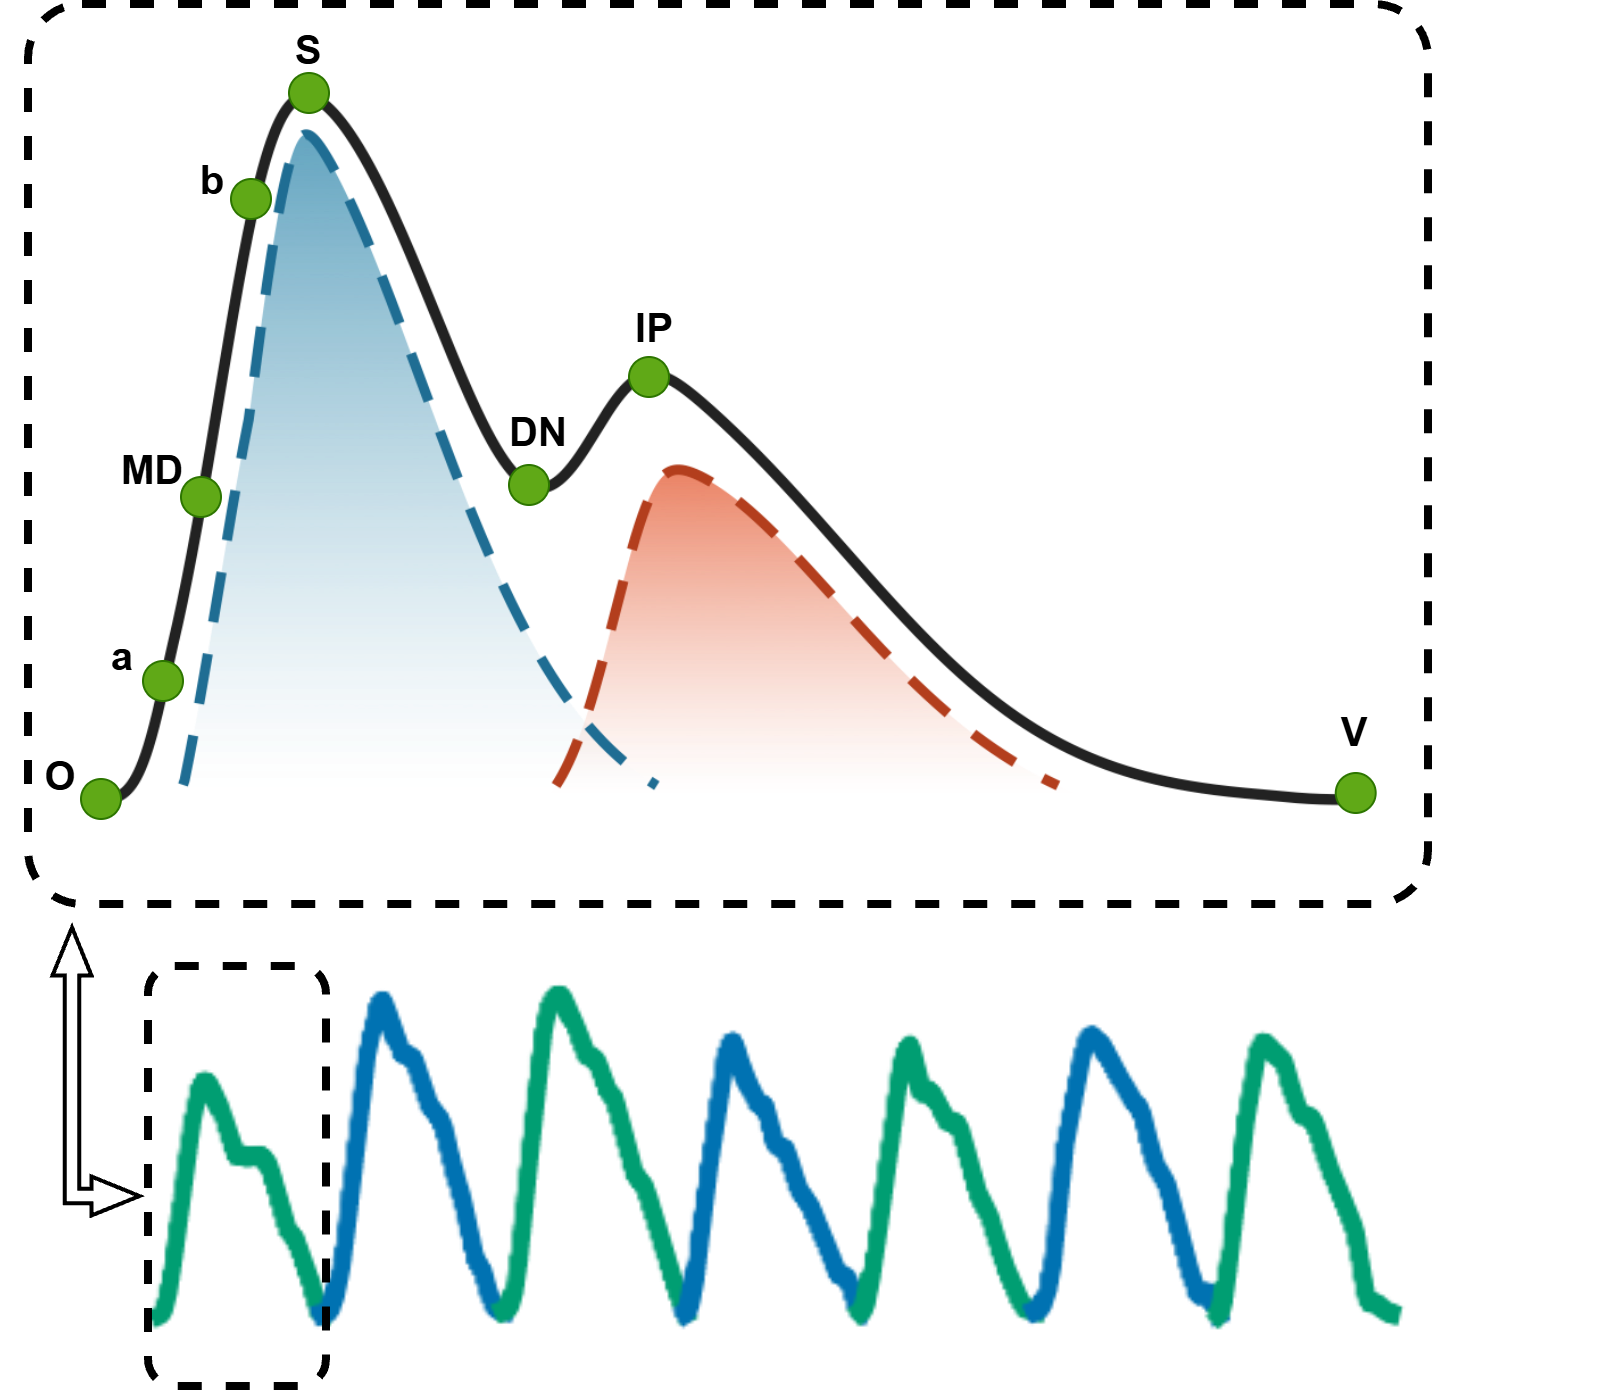
\includegraphics[width=\columnwidth]{3_生理学基础及信号特征/ppg_feat.drawio.png}
\caption{PPG 波形与基准点。单周期波形可视为前向波（蓝）与外周反射波（橙）叠加的结果，黑色曲线为单周期波形；特征点中O为收缩期起点、S 为主峰、DN 为重搏切迹、IP 为由反射波形成的次峰。}
\label{fig:ppg_wave}
\end{figure}

\subsection{与血压的生理关联}
\label{sec:ppg_bp}

PPG 信号本身携带心血管信息，这些信息隐含在波形之中，并可由上述特征反映出来。具体到血压任务，其物理基础在于波的传播：脉搏波沿动脉树传至外周再反射回来，波速由管壁弹性决定，血压升高时管壁张力增大、波速加快，反射波提前返回并在收缩期与前向波叠加，使切迹上移。

一些 PPG 形态学参数具有明确的生理学含义：次峰与主峰的幅度之比即反射指数（reflection index, RI），反映外周血管的反射强度，随年龄与血管状态系统性变化；上升时间与上升支斜率反映心室射血速度与动脉顺应性；主峰幅度、曲线下面积与 AC/DC 灌注指数则与每搏输出量和外周灌注水平相关\cite{millasseau2006contour,allen2007photoplethysmography,elgendi2019use}。时间维度上则是脉搏波传导时间（pulse transit time, PTT）：血压升高时波速加快、PTT 缩短，二者呈负相关，早期研究据此在间歇校准下连续估计收缩压\cite{chen2000continuous,poon2005cuffless}。只用单路 PPG 时，可用两峰间期 $\Delta T$（主峰至次峰的时间）作为波速的替代量——它对应脉搏波在主动脉与外周反射点之间的往返行程，与波速成反比，大动脉硬化时随之缩短\cite{millasseau2006contour}。这些参数与收缩压、舒张压确实存在统计相关，但相关强度受血管张力、体温、体位、呼吸与交感神经活动的调制，个体间差异显著，同一个体在不同时段的映射也会漂移\cite{lin2020investigating,yang2020estimation}。

综上，这些参数的生理含义虽然明确，但其与血压的相关强度随生理状态与个体而变，因此二者之间并不存在确定性的物理方程，只存在统计关系。基于此，血压估计被归结为一个映射学习问题：由一段 PPG 波形（或其派生特征）回归收缩压与舒张压，必要时还需要借助血压基线完成个体校准；用哪些特征也不能靠人工设计一劳永逸，而要由模型从数据中自行学习。这一转变构成\cref{sec:techniques}的主线。

